\chapter{Revised Plan}
\label{ch:plan}

Extra time has been allocated to update the type checking phase of Minigent in order to deal with
adding extra typechecking measure to \textsf{take} and \textsf{put}, in exchange of the time
needed to add type inference to remove \textsf{roll} and \textsf{unroll}. To complete this,
we must finalise the work in the type checker to automatically \textsf{roll}/\textsf{unroll} recursive type expressions
as explained in \autoref{sec:typecheckingprogress}. The updated timeline for the plan can be seen in \autoref{fig:revisedplan}.

As we no longer need to infer the use of \textsf{roll} and \textsf{unroll}, we have gained an extra
few weeks to work on the extensions for the project outlined in \autoref{sec:proposedextensions}.

\begin{figure}
    \centering
    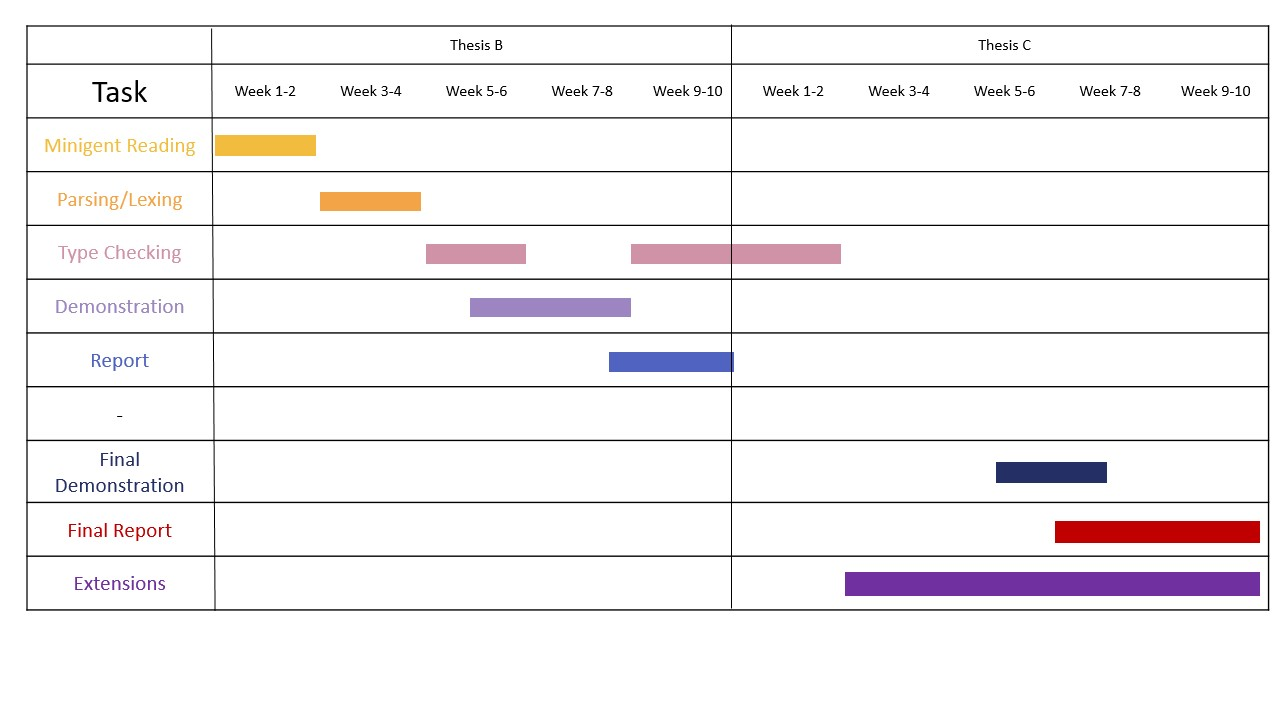
\includegraphics[height=0.50\textheight, angle=90]{content/revised_plan.jpg}
    \caption{The timeline for the project}
    \label{fig:revisedplan}
\end{figure}

The most important extension is to add primitive recursion detection for functions marked by
a \textsf{primrec} keyword, so that the programmer can get a guarantee from Cogent that
a function terminates before considering any kind of proof of termination.

A perhaps better design of this extension is to force all functions to require a termination guarantee
\textit{by default} or otherwise result in a compiler error, and allow use of a keyword e.g. \textbf{dangerous}
if the programmer wishes to acknowledge the function they wrote requires a manual proof of termination, or
may not even terminate at all.

This would allow programmers increased proof-concious development while writing Cogent code,
and upon integration with the Cogent embedding, a potential termination proof for free for
functions that Cogent can guarantee are primitive recursive.

\citet{AboutPrimrecAlgorithms}, in his paper on primitive recursive algorithms describes
an inductive definition of primitive recursive functions:

\theoremstyle{definition}
\begin{definition}
    \label{def:primrec}
    A function is \textit{primitive recursive} if it can be constructed using 
    a combination of the following combinators:

    \begin{itemize}
        \item 
            \textsf{O}, the \textit{null} or \textit{constant} combinator that takes zero arguemnts.
        \item 
            \textsf{Succ}, the \textit{successor} combinator that takes one argument, and returns the successor
            of that argument.
        \item 
            \textsf{$\pi^n_i$}, the \textit{projection} combinator that takes $n \geq 1$ arguments and returns
            the $i$'th argument, where $1 \leq i \leq n$.
        \item 
            \textsf{$S^n_m(f, g_1, g_2, \dots, g_n)$}, the \textit{composition} combinator, where $f$ and $g_{1..n}$ are 
            primitive recursive combinators that take $n$ and $m$ arguments respectfully, such that 
                $$S^n_m(f, g_1, g_2, \dots, g_n) = f(g_1(x_1, \dots, x_m), \dots, g_n(x_1, \dots, x_m))$$
        \item 
            \textsf{$Rec(b,s)$}, where $b$ and $s$ are primitive recursive combinators that take
            $n + 1$ arguments and $n + 2$ arguments respectfully is the \textit{recursion}
            combinator with base case $b$ and recursive step $n$.
    \end{itemize}
\end{definition}

In addition to a means to translate our Cogent programs into the above combinators,
we seek a method to map expressions to natural numbers that the above combinators can
operate on. Constructing this mapping correctly is a proof that our function is primitive recursive and
therefore terminates, otherwise however gives us no information about our function.

Whilst this extension may work for the class of primitive recursive functions, there are functions that
cannot be constructed using the primitive recursive axioms, for example the \textit{Ackermann Function}
\citep{Ackermann}. Therefore, detecting only primitive recursive functions limits the number of functions that
can obtain an automatic termination proof from Cogent to a small subset.

In conjunction with the primitive recursive approach, we may consider using
structurally recursive methods as discussed by \citet{StrucrecStructures} and \citet{PredicateStructrec}.
In this case our goal is to find a \textit{termination order} upon which our functions terminate --- An ordering
where each recursive call operates on arguments that are `smaller' than the previous, and prove 
that our recursion gradually terminates for a given input. 
As we don't have infinite objects in our recursive types due to their strictly positive condition, 
we know that are datatypes are finite in size, so functions that are  structurally recursive must
merely descend on the structure of the datatype, as measured by our termination order.

\citet{PredicateStructrec} talk in particular about \textit{structural ordering}, by measuring term size in
terms of constructors. They describe two axioms to measue this order, the first being given
a term $e$ and a constructor $C$, the transitive closure of:
$$
    e < C (\dots, e, \dots)
$$
And for measuring the size of function expressions, given a function $f$ of type $\alpha \longrightarrow \tau$,
and an argument $a$ of type $\alpha$:
$$
    f\; a \leq f
$$
Where the justification for this comes from set theory --- as a function is represented as the set of all pairs of
arguments and results, the result of one function application ($f\; a$) is less than or equal to the set of
all possible results ($f$).

With this means to order expressions in our language, we may apply various techniques for finding a termination
order - such as finding a \textit{lexicographical order} on the arguments of the function or measuring the \textit{size change}
of the arguments in the recursive calls of the function. Being able to construct a means to do this
mechanically will allow the Cogent typechecker to automatically find a termination proof for a certain subclass
of functions, allowing the resulting Isabelle embedding to contain free proofs about the termination of functions in this subclass. 